% Projeckt z předmětu INC
% Autor: Martin Slezák

\documentclass{article}

\usepackage[czech]{babel}
\usepackage{pdflscape}
\usepackage[letterpaper,top=2cm,bottom=2cm,left=3cm,right=3cm,marginparwidth=1.75cm]{geometry}

% Useful packages
\usepackage{amsmath}
\usepackage{graphicx}
\usepackage[colorlinks=true, allcolors=blue]{hyperref}

\title{Výstupní zpráva}
\author{Martin Slezák \\ xsleza26}
\date{\today}

\begin{document}
\maketitle

	% RTL circuit
	\section{Architektura navrženého obvodu}

	\subsection{Schéma obvodu}
	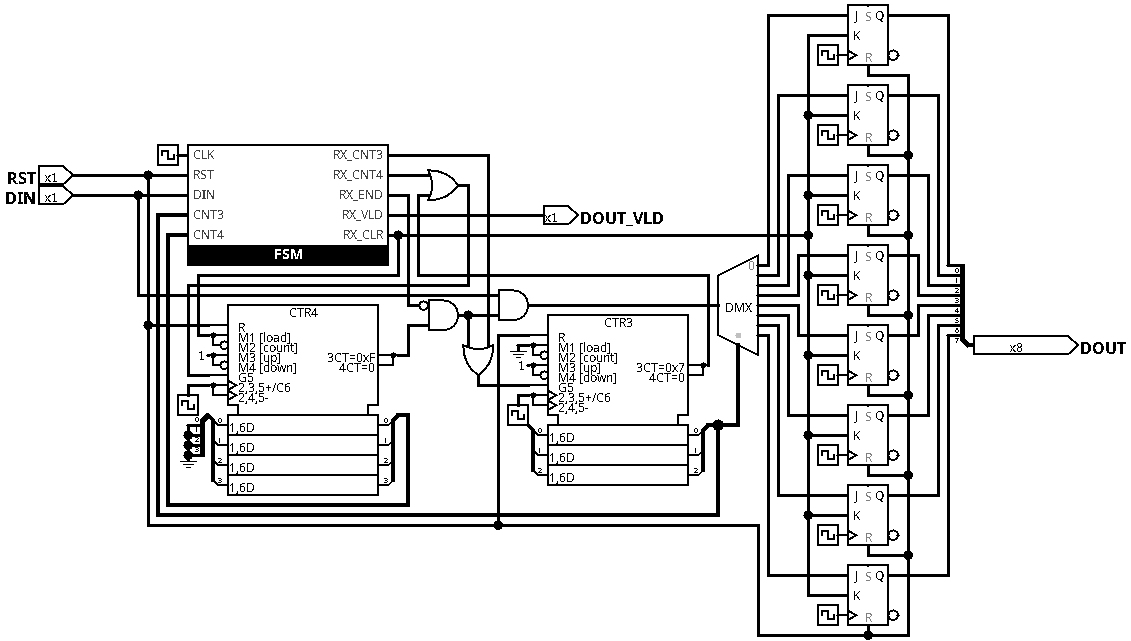
\includegraphics[scale=0.4]{"./src/rlc.png"}

	\subsection{Popis obvodu}
	\begin{itemize}
		\item Počítadlo CTR3 slouží pro offset 8 ticků (prostředek bitu) a pro výpis na
				jednotlivé bity
		\begin{itemize}
			\item Jakmile je výstup FSM RX\_CNT3 v logické jedničce,
					počítadlo počítá
			\item Při hodnotě 15 na počítadlu CTR4 se přičte jedna
		\end{itemize}

		\item Počítadlo CTR4 slouží pro čekání 16 ticků (čtení jednotlivých bitů)
		\begin{itemize}
			\item Jakmile je výstup FSM RX\_CNT4 v logické jedničce,
					počítadlo počítá
			\item Při hodnotě 7 na počítadlu CTR3 se přičte jedna
		\end{itemize}

		\item Demultiplexor slouží pro výpis hodnoty DIN na daný bit
				výstupu DOUT
		\begin{itemize}
			\item Vstup je hodnota DIN, v případě nastavení výstupu FSM
					RX\_END je vstup logická nula
			\item Vstup Select je výstup počítadla CTR3, které určuje, na
					který bit se zapisuje
		\end{itemize}

		\item Hodnoty výstupu se uchovávají pomocí JK klopného obvodu
		\item Výstup FSM RX\_VLD určuje platnost výstupu
		\item Výstup FSM RX\_CLR vynuluje JK klopné obvody a počítadlo CTR4
	\end{itemize}

	\newpage

	%Finite State Machine
	\section{Návrh automatu}

	\subsection{Schéma automatu}

	\subsubsection{Legenda:}
	\begin{itemize}
		\item \textbf{Stavy automatu:} WAIT\_START, WAIT\_OFFSET,WAIT\_READ,
				WAIT\_END, DATA\_VALID, WAIT\_END\_OFFSET
		\item \textbf{Vstupní signály:} CLK, RST, DIN, CNT3, CNT4
		\item \textbf{Mealyho výstupy:} žádné
		\item \textbf{Moorovy výstupy:}RX\_CNT3, RX\_CNT4, RX\_END,
				RX\_VLD, RX\_CLR (implicitní hodnoty v logické nule)
	\end{itemize}

	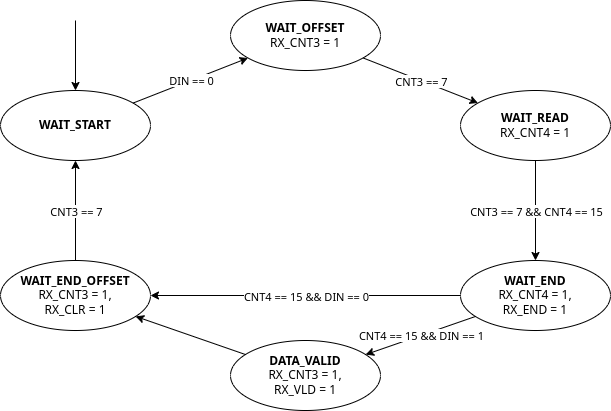
\includegraphics[scale=0.69]{./src/automat.png}

	\subsection{Popis automatu:}
	\begin{itemize}
		\item Vstupní stav je WAIT\_START, který čeká, než na vstupu DIN 
				bude logická nula
		\item WAIT\_OFFSET odpočítá 8 ticků offset pro čtení (prostředek bitu)
		\item WAIT\_READ přečte 8 bitů ze vstupu každých 16 ticků
		\item WAIT\_END počká 16 ticků (prostředek stop bitu)
		\item Jestli je nalezen stop bit (logická jednička), nastane 
				stav DATA\_VALID, v opačném případě bude nastaven stav
				WAIT\_END\_OFFSET
		\item V případě stavu DATA\_VALID se po jednom ticku přepne 
				na stav WAIT\_END\_OFFSET
		\item WAIT\_END\_OFFSET čeká 8 ticků, aby dočetl celý stop bit
	\end{itemize}


	\begin{landscape}
		\section{Snímek obrazovky se simulací}
		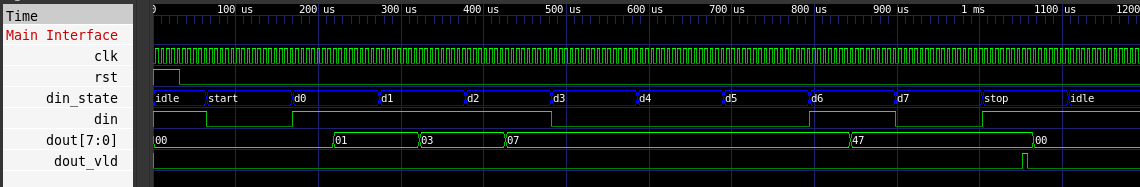
\includegraphics[scale=0.5953]{./src/simulation.png}
	\end{landscape}
\end{document}

%%%%% Projekt z předmětu IEL %%%% 
%% Autor: Martin Slezák

%\documentclass[]{fitiel}
%\usepackage{svg}

% implicitní cesta k obrázkům
%\graphicspath{{fig/}}

% hlavička 
% příkaz logo - vkládá logo fakulty dle zvoleného jazyka
%\title{\logo\\IEL -- protokol k projektu}
%\author{Martin, Slezák \\ xsleza26}
%\date{\today} % today - dnešní datum

%\begin{document}
%	\maketitle
	
%	\tableofcontents
	
%	\newpage
	
%\end{document}
